% Section 7: Simulation
\subsection{Simulation: decision-focused forecasting under AR(1) demand}
\label{sec:forecasting_rl_sim}

A clean synthetic instance makes the chapter's empirical claim concrete on
a substrate that an econometrician would recognise. The DGP is the
contextual AR(1) demand
\begin{equation}
y_t = \mu + \phi (y_{t-1} - \mu) + \beta^\top x_t + \sigma_t\,
\varepsilon_t, \qquad \varepsilon_t \sim \mathcal N(0, 1),
\label{eq:ar1_dgp}
\end{equation}
with $x_t \in \mathbb R^{10}$ drawn i.i.d.\ standard normal, persistence
$\phi = 0.7$, demand mean $\mu = 10$, and a heteroscedastic noise scale
$\sigma_t = \sigma_0 \exp(\gamma^\top x_t)$ with $\sigma_0 = 1$ and a
per-seed $\gamma$. The hypothesis class assumes homoscedasticity, so the
heteroscedasticity is the misspecification axis. The newsvendor cost
parameters of Section~\ref{sec:forecasting_rl_intro} carry over.
$c_u = 4$, $c_o = 1$, $\tau^\star = 0.8$. Each procedure trains on
$T = 2{,}000$ in-sample periods and evaluates on $500$ out-of-sample
periods, averaged over $20$ paired random seeds.

Three procedures share the AR(1)-plus-linear hypothesis class.
\emph{Method A} fits $(\mu, \phi, \beta, \sigma)$ by ordinary least
squares and plugs the fitted Gaussian distribution into the critical
fractile $q^{\mathrm A}_t = \hat\mu + \hat\phi (y_{t-1} - \hat\mu) +
\hat\beta^\top x_t + \hat\sigma\, \Phi^{-1}(\tau^\star)$. This is the
classical estimate-then-optimise pipeline. \emph{Method B} trains the
same parametric family by stochastic gradient descent on the SPO$^+$
surrogate of \citet{ElmachtoubGrigas2022} applied to the newsvendor loss,
and uses the same plug-in formula at decision time. \emph{Method C} takes
the OLS mean prediction and replaces the parametric residual quantile
$\hat\sigma\, \Phi^{-1}(\tau^\star)$ with the empirical residual quantile,
which is the simplest one-step rollout in the spirit of
\citet{BertsekasRollout2022}.

\begin{table}[h]
\centering
\caption{Decision-focused forecasting under AR(1) demand with
heteroscedastic noise, $20$ seeds, standard errors in parentheses.
Method B attains the same in-sample MSE as Method A but a factor-of-five
lower realised newsvendor regret.}
\label{tab:forecasting_rl_sim}
% Generated by decision_focused_ar1.py
\begin{tabular}{lccc}
\hline\hline
Method & In-sample MSE & Out-of-sample MSE & Mean newsvendor regret \\
\hline
A: OLS + critical fractile & $44.913\,(18.696)$ & $530.014\,(498.341)$ & $2.819\,(0.670)$ \\
B: Task-loss fine-tune & $45.646\,(18.789)$ & $529.350\,(497.261)$ & $0.597\,(0.142)$ \\
C: Bertsekas rollout & $44.913\,(18.696)$ & $530.014\,(498.341)$ & $0.946\,(0.177)$ \\
\hline\hline
\end{tabular}

\end{table}

\begin{figure}[h]
\centering
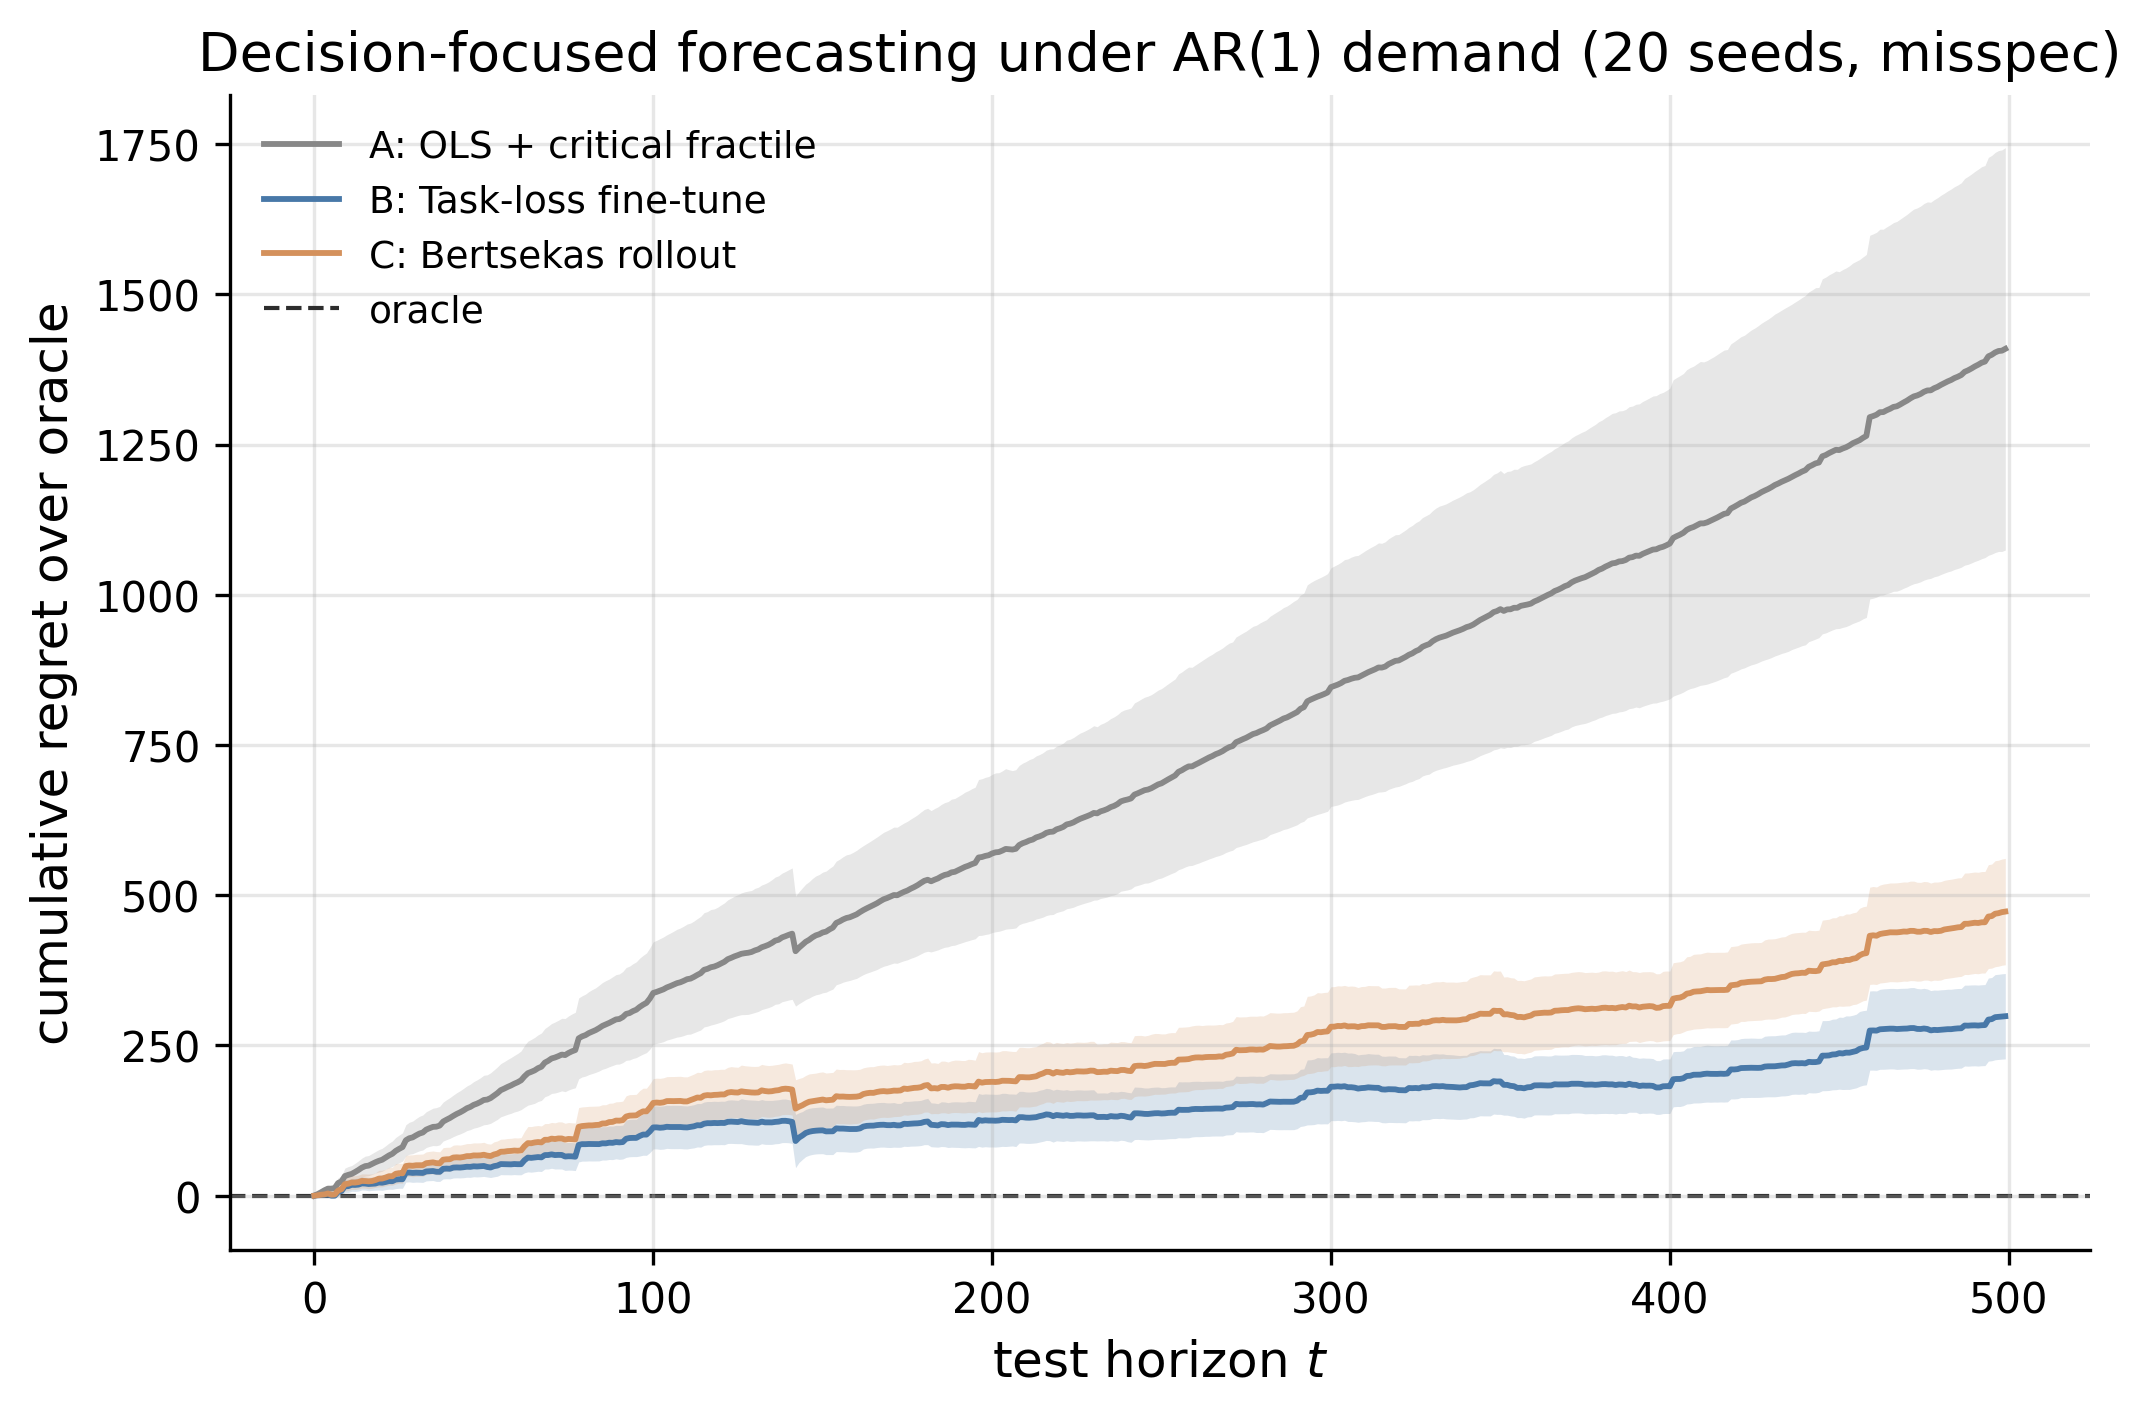
\includegraphics[width=0.85\linewidth]{../ch12_forecasting_rl/sims/decision_focused_ar1.png}
\caption{Cumulative newsvendor regret over the test horizon, $20$ seeds.
The shaded band is one standard error of the mean. The horizontal line at
zero is the oracle. Method B (SPO$^+$ fine-tune) attains the lowest
regret; Method A (OLS plus critical fractile) the highest.}
\label{fig:forecasting_rl_sim}
\end{figure}

Table~\ref{tab:forecasting_rl_sim} reports the realised costs. Method A's
in-sample MSE is $44.91 \pm 18.70$. Method B's is $45.65 \pm 18.79$,
statistically indistinguishable. Method C inherits Method A's MSE by
construction. The MSE ranking declares the three forecasters equivalent.
The realised newsvendor regret over $500$ test periods diverges sharply.
Method A's mean regret is $2.82 \pm 0.67$, Method B's is $0.60 \pm 0.14$,
and Method C's is $0.95 \pm 0.18$. Method B's regret is a factor of $4.7$
lower than Method A's, and Method C's is a factor of $3.0$ lower, both
with standard errors that exclude zero. Figure~\ref{fig:forecasting_rl_sim}
plots the cumulative regret over the test horizon.

The pattern is the Granger-Pesaran phenomenon of Section~\ref{sec:bridge}
on a familiar substrate. The MSE ranking and the decision-induced ranking
disagree once the noise model is misspecified, and a forecaster that
trades off in-sample squared error for in-sample realised cost wins on
realised cost out of sample. The simulation is also a worked example of
the \citet{HuKallus2020} counterpoint. Under well-specification with
$\gamma = 0$ the three methods are indistinguishable on regret as well as
on MSE, so the case for decision-focused training and rollout is
conditional on the heteroscedasticity that the homoscedastic OLS model
cannot represent.

The recipe extends naturally to sequential and to non-stationary settings.
Online decision-focused regret bounds at rate $T^{-1/4}$ exist under a
margin condition on the decision polytope \citep{Capitaine2025}, and the
extension to action-conditional foundation forecasters that an
economist's downstream-decision problem might require remains a research
frontier. The chapter's central methodological claim is unchanged. Two
forecasts that look identical on a strictly proper marginal loss can
differ by a substantial multiplicative factor on realised decision cost
whenever the noise model is misspecified or the cost structure is
asymmetric, and the corrective is a training objective that knows about
the decision.
